\subsection{Sound feature extraction}
Numerical representations of sound waves form the basis for audio features that allow algorithms to process and analyze sound beyond human perception. It is, therefore, important to extract these features as they have a bearing on how accurate and efficient the sound classification systems turn out. For classification of ultrasonic sounds emitted by plants that can be very complex, it is important to identify a set of features that accurately represent its characteristics.


\subsubsection{Mel Frequency Cepstral Coefficients (MFCC's)}
Mel Frequency Cepstral Coefficients (MFCCs) is a feature commonly used in speech and audio processing. This section explains what MFCCs are, why they’re used, and how they’re calculated.

\paragraph{Theoretical background}
The human ear's cochlea vibrates at different spots depending on the incoming sounds’ frequencies. This vibration can be modeled as a filter bank with triangular filters starting from low frequencies and moving upwards logarithmically until the highest ones are reached (Mel scale). The concept behind this non-linear frequency scale lies on how lower frequencies seem more easily distinguishable than higher ones by human ears. \cite{casale_physiology_2024}

Mel-frequency cepstrum coefficients are representations of the power spectrum of a sound in short time intervals. The term “cepstrum” derives from reversing the first four letters of “spectrum.” While normal cepstral representations work fine for some applications, MFCC's are designed to mimic the human ear's response more closely than the linearly-spaced frequency bands in order to better mimic the human ear’s response. This mimicking behavior is especially necessary for tasks like speech recognition or music analysis as well as feature extraction from those parts of acoustic spectrum where some sounds like plants produce frequencies outside normal hearing ranges. \cite{noauthor_mel-frequency_2024}


\textbf{Computational Process} \cite{gupta_feature_2013, zater_feature_2022}

\begin{figure}
    \centering
    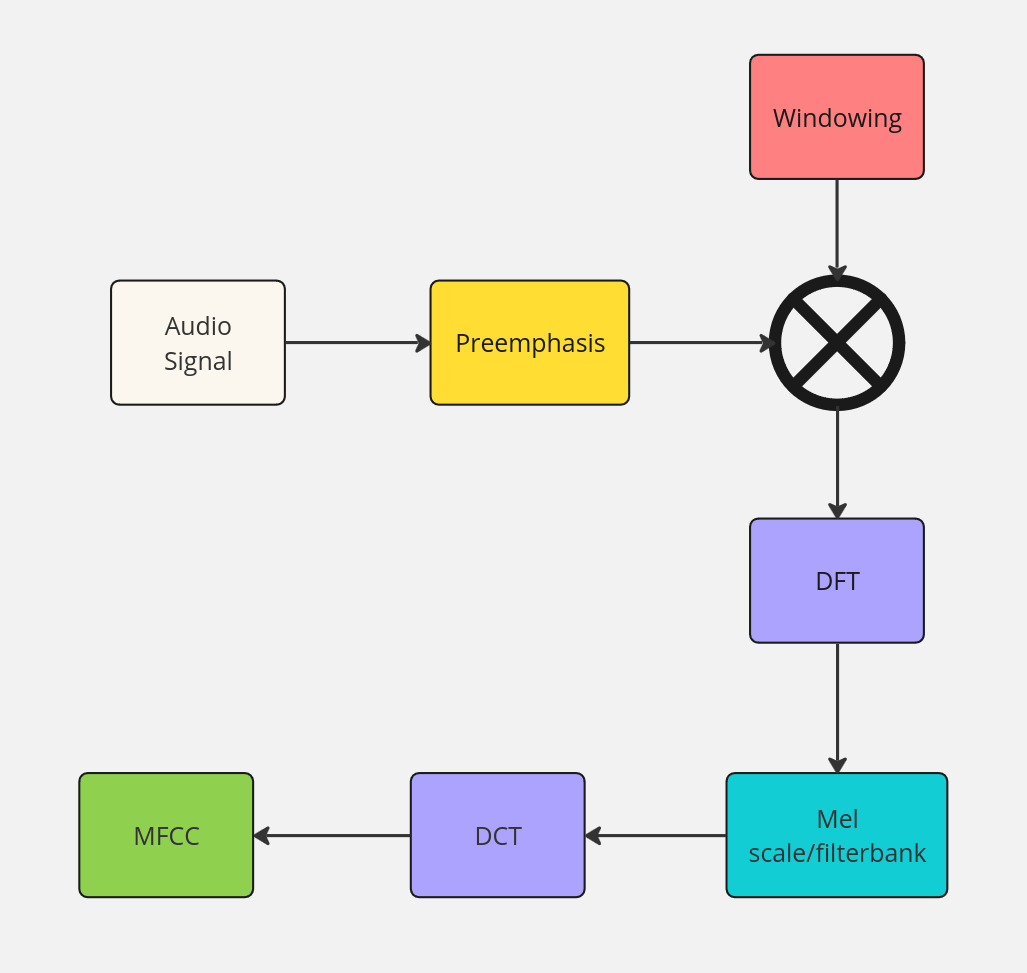
\includegraphics[width=0.5\linewidth]{images/mfcc_Flowchart.jpg}
    \caption{flowchart illustrating the fundamental process for computing Mel Frequency Cepstral Coefficients (MFCCs)}
    \label{fig:enter-label}
\end{figure}

\begin{enumerate}
    \item \textbf{Pre-emphasis:}
    The signal goes through an amplifyer to boost high frequencies in order to compensate for the decrease in magnitude at higher ones during recording.

    \item \textbf{Windowing:}
    The signal is sliced into short time frames. Windowing helps to minimize the signal discontinuities at the beginning and end of each frame. The window function, like a Hamming window, is typically applied to each frame to reduce the signal discontinuities at the boundaries.

    \item \textbf{DFT (Discrete Fourier Transform):}
    The Fourier Transform converts each frame of windowed signal from time domain to frequency domain, creating a spectrum for each frame.

    \item \textbf{Mel Filterbank:}
    Power spectrogram obtained from the DFT are then passed through a set of filters that simulates the non-linear human ear perception of pitch. Triangular and evenly spaced on the Mel scale.

    \item \textbf{Discrete Cosine Transform (DCT):}
    Finally, the log Mel spectrum is converted back into time domain by Discrete Cosine Transform, resulting in a time-domain representation of frequency information for each frame as a vector.
\end{enumerate}



MFCCs are used in various audio processes and machine learning tasks, particularly in speech recognition systems. Their ability to capture key features of human speech and the ear’s response makes them useful for distinguishing linguistic content and speaker characteristics in sound signals. They’ve been applied for voice recognition, music genre classification, emotion detection, and many other instances where sound is involved. \cite{zater_feature_2022}

Their use to classify plant sounds, specifically ultrasonic emissions that result from plants being under stress, is a new path of research. Plants produce a range of sounds in response to environmental threats, some of which fall outside our hearing abilities, so MFCCs’ accuracy and flexibility would be ideal. Analyzing these ultrasonic emissions could give researchers an understanding of plant health and stress levels, opening new doors in farming monitoring and care. \cite{Cell_Sounds_emitted_by_plants}

\subsubsection{Deep Scattering Spectrum (DSS)}
The Deep Scattering Spectrum (DSS) technology \cite{anden_deep_2014}, developed by Joakim Andén and Stéphane Mallat, represents a groundbreaking advancement in the audio classification domain. It is based on a mathematical framework of scattering transforms that allows for extraction of stable and invariant features from complex audio signals in an efficient manner.

DSS works by using scattering transform which is an extension of Mel-frequency cepstral coefficients (MFCCs), whereby modulation spectrum coefficients are integrated through multiple orders. This process consists of cascaded operations of wavelet convolutions and modulus operators. While traditional Fourier-based analyses may not be able to handle deformations such as time warping common in audio signals, scattering transforms are stable to time deformations while their local translation invariance remains intact.\cite{anden_deep_2014}

The second-order scattering coefficients are the core of the DSS method. Their job includes capturing transient events within audio; sudden attacks or amplitude modulations, which help distinguish complex sound patterns. The procedure starts with an initial wavelet transform followed by a modulus operation to obtain envelope information without losing energy over scales. Subsequent layers consist of wavelet transformations and modulus operations that reveal higher order features containing rich temporal and spectral information.\cite{anden_deep_2014}

DSS finds application within several realms of audio signal processing. DSS outperforms classical MFCC based techniques when it comes to musical genre classification since it captures wide range of audio characteristics leading to accurate identification of the genre. Due to its ability to identify subtle modulations and transient sounds even under noisy conditions, it is superior in classification for speech recognition purposes. An additional example can be seen in environmental sound analysis where distinguishing between complicated soundscapes is accomplished with ease by DSS. Ecosystem monitoring or urban sound classification would benefit from this sort of differentiation used for complex soundscapes. \cite{anden_deep_2014}

The study on ultrasonic sounds emitted by tomato and tobacco plants \cite{Cell_Sounds_emitted_by_plants} subjected to drought stress and physical injury were recorded and analyzed. It was possible for machine learning models trained using the scattering network features for differentiating between stressed and non-stressed plants thereby demonstrating that this method works in real life situations. Furthermore, this approach is also able not only to detect plant stress but also determine what kind of stress like dehydration or tissue damage.






